% =====================================================================
%  Teorema di continuità del limite -- lezione 2
% =====================================================================

% [0:02:47]
\section{Teorema di continuità del limite}

\paragraph{In aula.} Fra le dimostrazioni viste oggi, quella del passaggio al limite
sotto il segno di integrale è indicata come possibile domanda d'esame; si dà per
noto tutto il materiale di Analisi I che vi compare (teorema di Weierstrass,
proprietà di confronto degli integrali, teorema dei carabinieri).

% [0:03:55]
\subsection{Enunciato}

La convergenza puntuale non conserva le proprietà delle funzioni che compongono la
successione: è proprio per questo che è stata introdotta la convergenza uniforme. Il
primo teorema che vediamo dice che, con la convergenza uniforme, la continuità si
trasmette al limite.

\Teorema{continuità del limite uniforme}{%
Siano
\begin{enumerate}
  \item $f_n\colon I\subseteq\mathbb{R}\to\mathbb{R}$ continua in $I$ per ogni $n$;
  \item $f_n\rightrightarrows f$ in $I$, con $f\colon I\subseteq\mathbb{R}\to\mathbb{R}$.
\end{enumerate}
Allora $f$ è continua in $I$.
}

% [0:05:50]
\BoxBlue{Osservazione}{}{%
Equivalentemente, la tesi si scrive come uno scambio di
limiti: per ogni $x_0\in I$
\begin{equation}
\lim_{x\to x_0} f(x)
= \lim_{x\to x_0}\Big(\lim_{n\to\infty} f_n(x)\Big)
= \lim_{n\to\infty}\Big(\lim_{x\to x_0} f_n(x)\Big)
= \lim_{n\to\infty} f_n(x_0)
= f(x_0).
\end{equation}
Nella prima uguaglianza si è usato che $f$ è il limite puntuale delle $f_n$, nella
terza che ciascuna $f_n$ è continua in $x_0$.
}

% [0:08:06]
\paragraph{In aula.} Il senso della formula precedente è questo: $f_n(x)$ dipende da
due variabili, l'indice $n$ e il punto $x$. In generale due operazioni di limite su
variabili diverse non si possono scambiare; \textbf{[In aula]} quando la convergenza
è uniforme, invece, i due limiti si possono invertire liberamente.

% [0:09:33]
\BoxBlue{Osservazione}{}{%
Il teorema \emph{non} è un ``se e solo se''. Se lo fosse,
lo studio della convergenza uniforme si ridurrebbe allo studio della continuità del
limite puntuale. Il controesempio è già noto: $f_n(x)=x/n$ converge puntualmente a
$f\equiv 0$, che è continua, ma la convergenza non è uniforme su tutto $\mathbb{R}$.
Quindi la continuità del limite puntuale non caratterizza la convergenza uniforme.
}

% [0:09:33]
\paragraph{In aula.} Il teorema si usa quasi sempre ``al negativo''. Se le $f_n$ sono
continue e il limite puntuale $f$ risulta discontinuo, allora si conclude
immediatamente che la convergenza \emph{non} è uniforme, senza calcolare alcun
$\sup$. È il caso di $f_n(x)=x^n$ su $[0,1]$ (figura~\ref{fig:01}), il cui limite
puntuale è
\[
f(x)=
\begin{cases}
0, & x\in[0,1[,\\[2pt]
1, & x=1.
\end{cases}
\]

\begin{figure}[htbp]\centering
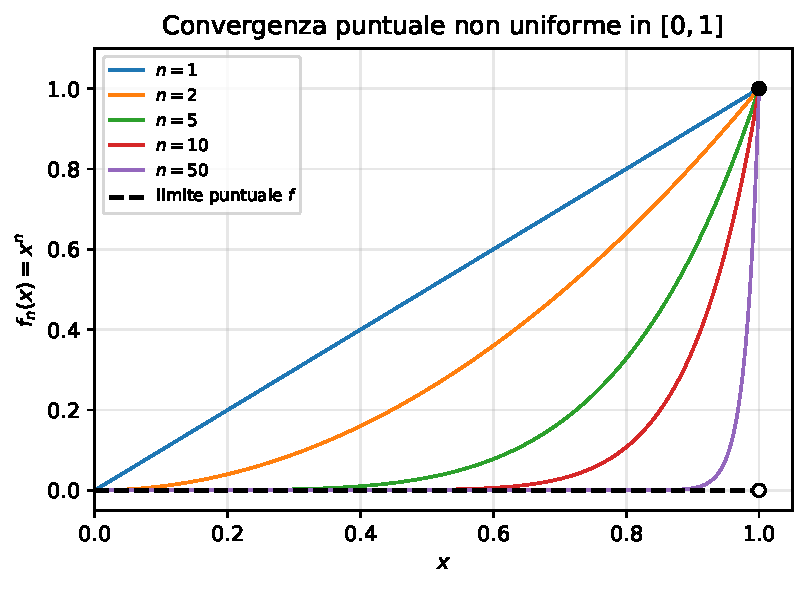
\includegraphics[width=0.6\linewidth]{figure/fig_01}
\caption{Andamento qualitativo di $f_n(x)=x^n$ su $[0,1]$ per alcuni valori di $n$ e
suo limite puntuale, discontinuo in $x=1$: essendo le $f_n$ continue, la convergenza
non può essere uniforme su $[0,1]$.}
\label{fig:01}
\end{figure}

% [0:10:34]
\paragraph{In aula.} Il teorema dice anche \emph{dove} conviene restringersi. Non
basta prendere un intervallo più piccolo a caso: su $[1/2,1]$ la discontinuità viene
di nuovo catturata e la convergenza resta non uniforme. Bisogna restringersi a un
insieme su cui il limite puntuale è continuo, per esempio $[0,a]$ con $a<1$. Questo è
il criterio pratico per cercare l'insieme più grande su cui si ha convergenza
uniforme.

% [0:11:43]
\subsection{Dimostrazione}

Sia $x_0\in I$; dimostriamo che $f$ è continua in $x_0$. Poiché $x_0$ è arbitrario,
seguirà la continuità su tutto $I$.

Dalle ipotesi:
\begin{itemize}
  \item dall'ipotesi 1, $f_n$ è continua in $x_0$, cioè
  \[
  \forall \epsilon>0 \;\; \exists\, \delta_n>0:\quad
  |f_n(x)-f_n(x_0)|<\epsilon \quad \forall x\in I,\ |x-x_0|<\delta_n;
  \]
  \item dall'ipotesi 2, $f_n\rightrightarrows f$ in $I$, cioè
  \[
  \forall \epsilon>0 \;\; \exists\, \nu_\epsilon>0:\quad
  |f_n(x)-f(x)|<\epsilon \quad \forall n>\nu_\epsilon,\ \forall x\in I.
  \]
\end{itemize}

\paragraph{In aula.} Nella prima definizione il $\delta$ dipende anche da $n$: ogni
$f_n$ ha il suo. Nella seconda, invece, l'indice $\nu_\epsilon$ è unico e va bene per
\emph{tutte} le $x$ contemporaneamente: è esattamente questo il contenuto in più
della convergenza uniforme, ed è l'unico ``ingrediente'' che serve ricordare della
dimostrazione.

Dobbiamo produrre il $\delta$ della continuità di $f$. Fissato $\epsilon>0$ partiamo
dalla quantità da stimare e inseriamo un termine $f_{\bar m}$ con
$\bar m>\nu_\epsilon$:
\begin{align*}
|f(x)-f(x_0)|
&= \big| f(x)-f_{\bar m}(x)+f_{\bar m}(x)-f_{\bar m}(x_0)+f_{\bar m}(x_0)-f(x_0)\big|\\
&\le \underbrace{|f(x)-f_{\bar m}(x)|}_{<\,\epsilon \ \text{per la 2}}
+\underbrace{|f_{\bar m}(x)-f_{\bar m}(x_0)|}_{<\,\epsilon \ \text{per la 1}}
+\underbrace{|f_{\bar m}(x_0)-f(x_0)|}_{<\,\epsilon \ \text{per la 2}}
\;<\;3\epsilon .
\end{align*}
Il primo e il terzo addendo si stimano con la convergenza uniforme (lo stesso indice
$\bar m$ va bene sia in $x$ sia in $x_0$); il secondo si stima con la continuità di
$f_{\bar m}$, che fornisce il $\delta_{\bar m}>0$ cercato. Poiché $\epsilon>0$ è
arbitrario, $f$ è continua in $x_0$. $\blacksquare$

\BoxBlue{Osservazione}{}{%
Se si preferisce ottenere esattamente $\epsilon$ al posto di
$3\epsilon$, basta applicare le tre stime con $\epsilon/3$.
}

\subsection{Un esempio con limite discontinuo in un punto}

\paragraph{Esempio.} Sia
\[
f_n(x)=\frac{\arctan\!\big(n(1+x^2)\big)}{1+n^2x^2}+x,
\qquad x\in[0,+\infty[.
\]
Il limite puntuale è
\[
\lim_{n\to\infty} f_n(x)=f(x)=
\begin{cases}
x, & x\in\,]0,+\infty[,\\[4pt]
\dfrac{\pi}{2}, & x=0,
\end{cases}
\]
perché per $x>0$ il numeratore resta limitato mentre il denominatore diverge, mentre
in $x=0$ resta $\arctan(n)\to\pi/2$. Il limite è discontinuo in $x=0$ e le $n$ sono
continue: per il teorema di continuità del limite non c'è convergenza uniforme su
$[0,+\infty[$ (figura~\ref{fig:08}).

Ci si restringe allora a $[a,+\infty[$ con $a>0$, dove il limite $f(x)=x$ è continuo.
Qui
\[
M_n=\sup_{x\in[a,+\infty[}\left|\frac{\arctan\!\big(n(1+x^2)\big)}{1+n^2x^2}\right|
\le \frac{\pi}{2}\,\sup_{x\in[a,+\infty[}\frac{1}{1+n^2x^2}
= \frac{\pi}{2}\cdot\frac{1}{1+n^2a^2}\longrightarrow 0,
\]
quindi $M_n\to 0$ per il teorema dei carabinieri e la convergenza è uniforme su
$[a,+\infty[$.

\BoxBlue{Osservazione}{}{%
La maggiorazione funziona perché l'arcotangente è
\emph{limitata}: si sostituisce il fattore scomodo con la sua limitazione $\pi/2$ e si
evita del tutto il calcolo esatto del $\sup$ (cioè lo studio della derivata).
}

\begin{figure}[htbp]\centering
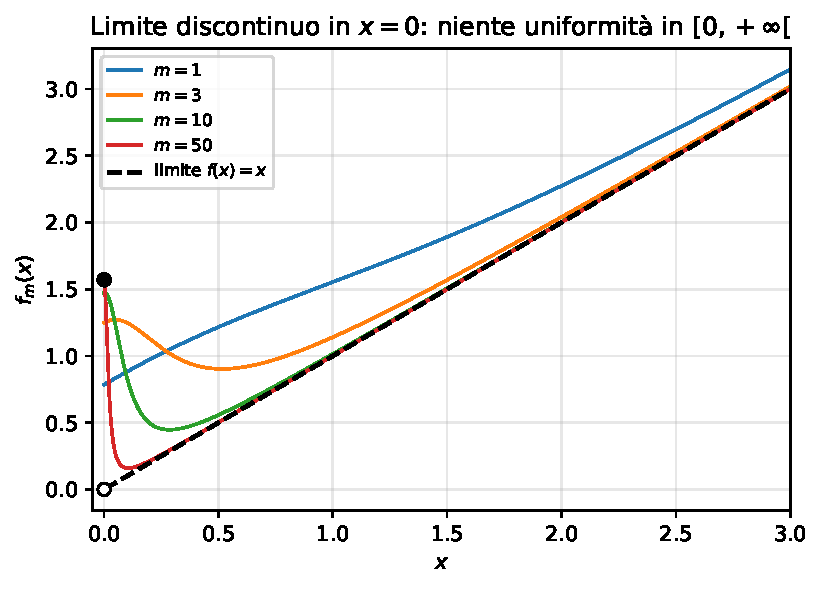
\includegraphics[width=0.6\linewidth]{figure/fig_08}
\caption{Andamento qualitativo di $f_n(x)=\arctan(n(1+x^2))/(1+n^2x^2)+x$ su
$[0,3]$: il limite puntuale vale $x$ per $x>0$ e $\pi/2$ in $x=0$.}
\label{fig:08}
\end{figure}

% [0:52:38]
\paragraph{In aula.} Un esercizio analogo, con lo stesso schema logico, è
$f_n(x)=\arctan(nx)$ su $\mathbb{R}$ (figura~\ref{fig:02}). Il limite puntuale è
\[
f(x)=
\begin{cases}
\pi/2, & x>0,\\
0, & x=0,\\
-\pi/2, & x<0,
\end{cases}
\]
discontinuo in $0$: niente convergenza uniforme su $\mathbb{R}$. Ci si può restringere
a $[a,+\infty[$ con $a>0$ \emph{oppure} a $]-\infty,-a]$ con $a>0$, ma non all'unione
dei due, perché l'insieme sarebbe sconnesso e si tornerebbe ad avere un limite
discontinuo [?]. Sul primo intervallo
\[
\sup_{x\ge a}\left|\arctan(nx)-\frac{\pi}{2}\right|
=\sup_{x\ge a}\left(\frac{\pi}{2}-\arctan(nx)\right)
=\frac{\pi}{2}-\arctan(na)\longrightarrow 0 .
\]
\textbf{[In aula]} Il valore assoluto si toglie scambiando i due termini (la
differenza ha segno costante) e il $\sup$ si trova \emph{senza} derivate: l'arcotangente
è crescente, quindi $\pi/2-\arctan(nx)$ è decrescente e il massimo si raggiunge
nell'estremo inferiore $x=a$. Il fatto che sia $a\neq 0$ è esattamente ciò che rende
il limite nullo.

\begin{figure}[htbp]\centering
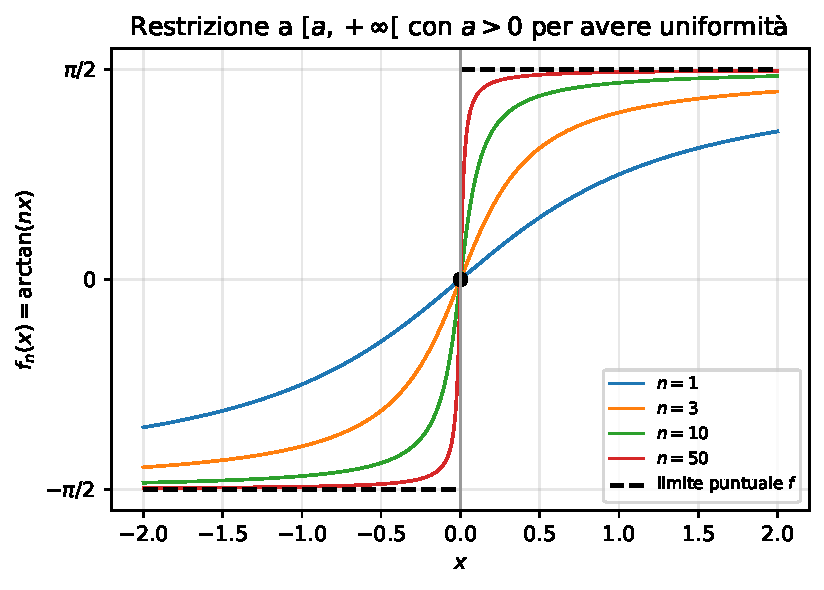
\includegraphics[width=0.6\linewidth]{figure/fig_02}
\caption{Andamento qualitativo di $f_n(x)=\arctan(nx)$: la convergenza è uniforme su
ogni $[a,+\infty[$ con $a>0$, ma non su $\mathbb{R}$.}
\label{fig:02}
\end{figure}
